\documentclass[11pt, a4paper]{article}

% ============================================================
% Packages
% ============================================================
\usepackage[utf8]{inputenc}
\usepackage[T1]{fontenc}
\usepackage{amsmath, amssymb, amsthm}
\usepackage{mathtools}
\usepackage{bm}
\usepackage{geometry}
\usepackage{hyperref}
\usepackage{cleveref}
\usepackage{algorithm}
\usepackage{algpseudocode}
\usepackage{graphicx}
\usepackage{booktabs}
\usepackage{multirow}
\usepackage{enumitem}
\usepackage{natbib}
\usepackage{xcolor}
\usepackage{tikz}
\usetikzlibrary{arrows.meta, positioning, shapes.geometric}

\geometry{margin=2.5cm}
\hypersetup{colorlinks=true, linkcolor=blue!70!black, citecolor=green!50!black, urlcolor=blue!60!black}

% ============================================================
% Theorem environments
% ============================================================
\newtheorem{theorem}{Theorem}[section]
\newtheorem{proposition}[theorem]{Proposition}
\newtheorem{lemma}[theorem]{Lemma}
\newtheorem{definition}[theorem]{Definition}
\newtheorem{remark}[theorem]{Remark}

% ============================================================
% Macros
% ============================================================
\newcommand{\R}{\mathbb{R}}
\newcommand{\E}{\mathbb{E}}
\newcommand{\Prob}{\mathbb{P}}
\newcommand{\Var}{\mathrm{Var}}
\newcommand{\Sig}{\mathrm{Sig}}
\newcommand{\MMD}{\mathrm{MMD}}
\newcommand{\dd}{\mathrm{d}}
\newcommand{\logp}{\log P}
\DeclareMathOperator{\softplus}{softplus}

\title{%
  \textbf{Neural Stochastic Differential Equations for Generative Stress-Testing of Cointegrated Pairs Trading Strategies}
}

\author{
  Killian Guillaume \\
  \textit{Independent Research} \\
  \texttt{killian.guillaume@email.com}
}

\date{\today}

% ============================================================
\begin{document}
% ============================================================

\maketitle

\begin{abstract}
We present a generative framework for stress-testing statistical arbitrage strategies on cointegrated asset pairs. 
The core model is a \emph{Neural Stochastic Differential Equation} (Neural SDE) that learns the joint dynamics of two log-price processes conditioned on a spread deviation signal encoding mean-reversion. 
The model is trained via a \emph{Kernel Maximum Mean Discrepancy} (MMD) loss computed on truncated path signatures, ensuring distributional convergence in the space of continuous paths rather than pointwise matching.
At inference, the trained SDE generates millions of synthetic market trajectories that preserve the cointegration structure, volatility clustering, and tail behavior of real data.
These synthetic paths are filtered via the Augmented Dickey--Fuller test and fed into a Monte Carlo backtesting engine that computes Value-at-Risk and Conditional Value-at-Risk under realistic transaction cost models.
We describe the full mathematical framework and the architectural design decisions that make this pipeline production-ready.
\end{abstract}

\vspace{0.5em}
\noindent\textbf{Keywords:} Neural SDE, Generative Model, Pairs Trading, Cointegration, Path Signatures, MMD, Stress Testing, Monte Carlo Simulation

% ============================================================
\section{Introduction}
\label{sec:intro}
% ============================================================

Pairs trading is a market-neutral strategy that exploits temporary deviations between two cointegrated assets \citep{vidyamurthy2004pairs}. 
A critical challenge is \emph{stress-testing}: evaluating whether a calibrated strategy is robust to unseen market conditions, liquidity crises, or regime changes. 
Historical backtesting is limited to a single realized path of the market, which provides no distributional information about strategy performance.

We address this limitation by building a \emph{Neural SDE}~\citep{kidger2021neural} that learns the joint stochastic dynamics of two cointegrated price processes. 
Once trained, the model generates arbitrarily many synthetic market trajectories, each preserving the cointegration relationship, while exhibiting natural variation in volatility, drift, and tail events.

Our key contributions are:
\begin{enumerate}[nosep]
    \item A 2-dimensional Neural SDE architecture with a \emph{spread deviation conditioning} mechanism that explicitly encodes mean-reversion inductive bias.
    \item Training via \emph{Kernel Signature MMD}, a distributional loss that matches the law of generated paths to real data in the universal feature space of path signatures.
    \item A production pipeline that combines the generative model with ADF-based quality filtering and Monte Carlo risk evaluation (VaR, CVaR) under 4 realistic cost scenarios.
\end{enumerate}

% ============================================================
\section{Problem Formulation}
\label{sec:problem}
% ============================================================

Let $P^A_t$ and $P^B_t$ denote the prices of two assets at time $t$. We work in log-price space, defining the state vector:
\begin{equation}
    X_t = \begin{pmatrix} \logp^A_t \\ \logp^B_t \end{pmatrix} \in \R^2.
\end{equation}

The \emph{log-spread} is defined as:
\begin{equation}
    s_t = \logp^A_t - \logp^B_t.
\end{equation}

For a cointegrated pair, $s_t$ is a stationary process. The trading signal is derived from the z-score of $s_t$, and the strategy enters when $|z_t| > \tau_{\text{entry}}$ and exits when $|z_t| < \tau_{\text{exit}}$.

\begin{remark}
Working in log-price space (rather than raw prices) ensures \emph{scale invariance}: the same model can generate paths for assets with vastly different nominal prices, since the SDE operates on dimensionless standardized log-prices.
\end{remark}

\subsection{Data Preprocessing}

Given raw price series $(P^A_t, P^B_t)_{t=1}^{T}$, we compute:
\begin{equation}
    \tilde{X}_t = \frac{X_t - \hat{\mu}}{\hat{\sigma}}, \quad
    \hat{\mu} = \frac{1}{T}\sum_{t=1}^T X_t, \quad
    \hat{\sigma} = \sqrt{\frac{1}{T}\sum_{t=1}^T (X_t - \hat{\mu})^2},
\end{equation}
where $\hat{\mu}, \hat{\sigma} \in \R^2$ are computed component-wise on the training set only. The validation set uses the training set's statistics to prevent information leakage.

\subsection{Strided Sampling}

Training sequences are extracted as sliding windows of length $L$ from the standardized time series. With a naïve stride of~1, consecutive windows $\tilde{X}_{t:t+L}$ and $\tilde{X}_{t+1:t+1+L}$ overlap by $L-1$ points, creating near-duplicate training samples that encourage memorization of micro-transitions rather than learning the underlying generative dynamics.

To enforce statistical independence between training samples, we subsample windows with a stride $\Delta > 1$:
\begin{equation}
    \mathcal{D}_{\text{train}} = \left\{\tilde{X}_{k\Delta : k\Delta + L}\right\}_{k=0}^{\lfloor (T-L)/\Delta \rfloor}.
\end{equation}

This reduces the dataset size by a factor of $\Delta$ but dramatically improves generalization: the model is forced to learn the \emph{distributional law} of the process (cointegration, volatility clustering) rather than memorizing specific sequences. In practice, $\Delta = 8$ provides a good trade-off between sample diversity and dataset size for hourly data.

% ============================================================
\section{Neural SDE Architecture}
\label{sec:model}
% ============================================================

\subsection{State-Space Formulation}

We model the joint dynamics of the standardized log-prices as an Itô SDE:
\begin{equation}
\label{eq:sde}
    \dd \tilde{X}_t = f_\theta\!\left(\tilde{X}_t,\, \Delta s_t\right) \dd t + g_\theta\!\left(\tilde{X}_t,\, \Delta s_t\right) \dd W_t,
\end{equation}
where:
\begin{itemize}[nosep]
    \item $\tilde{X}_t \in \R^2$ is the SDE state (standardized log-prices of assets A and B),
    \item $f_\theta : \R^3 \to \R^2$ is the \emph{drift network} (parametric trend),
    \item $g_\theta : \R^3 \to \R^2_{>0}$ is the \emph{diffusion network} (parametric local volatility),
    \item $W_t \in \R^2$ is a standard 2-dimensional Brownian motion (diagonal noise),
    \item $\Delta s_t$ is the \emph{spread deviation} signal defined below.
\end{itemize}

\subsection{Spread Deviation Conditioning}

Rather than feeding the raw spread $s_t = \tilde{X}_t^{(1)} - \tilde{X}_t^{(2)}$ to the networks, we use the \emph{deviation from the initial spread}:
\begin{equation}
\label{eq:spread_dev}
    \Delta s_t = s_t - s_0 = \left(\tilde{X}_t^{(1)} - \tilde{X}_t^{(2)}\right) - \left(\tilde{X}_0^{(1)} - \tilde{X}_0^{(2)}\right).
\end{equation}

This design choice introduces mean-reversion inductive bias: $\Delta s_0 = 0$ at integration start, and the drift network observes only the \emph{tension} (how far the spread has moved from its starting point), not its absolute level. This encourages the drift to learn a restoring force that pulls $\Delta s_t$ back toward zero.

The extended input to both networks is:
\begin{equation}
    \tilde{X}_t^{\text{ext}} = \left(\tilde{X}_t^{(1)},\, \tilde{X}_t^{(2)},\, \Delta s_t\right) \in \R^3.
\end{equation}

\subsection{Network Architectures}

Both $f_\theta$ and $g_\theta$ are implemented as 3-layer MLPs with SiLU activations:
\begin{align}
    f_\theta &: \R^3 \xrightarrow{\text{Linear}(3, H)} \xrightarrow{\text{SiLU}} \xrightarrow{\text{Linear}(H, H)} \xrightarrow{\text{SiLU}} \xrightarrow{\text{Linear}(H, 2)} \R^2, \\
    g_\theta &: \R^3 \xrightarrow{\cdots \text{(same architecture)}} \xrightarrow{\softplus} \R^2_{>0},
\end{align}
where $H$ is the hidden dimension (64 in our experiments). We rely on strided sampling (Section~\ref{sec:problem}) and weight decay rather than dropout for regularization, since dropout introduces stochasticity in the drift and diffusion functions that can destabilize the SDE solver during integration.

\paragraph{Weight initialization.}
To ensure stability at the start of training:
\begin{itemize}[nosep]
    \item $f_\theta$: last layer weights and biases initialized to zero (zero drift at $t=0$).
    \item $g_\theta$: last layer bias initialized to $\softplus^{-1}(\sigma_{\text{target}})$ to match a target volatility level.
\end{itemize}

\paragraph{Positivity of diffusion.}
The softplus activation $\softplus(x) = \log(1 + e^x)$ guarantees $g_\theta > 0$. An additional clamp $g_\theta \in [\sigma_{\min}, 5.0]$ prevents both numerical underflow and explosion during integration.

\subsection{Numerical Integration}

The SDE \eqref{eq:sde} is solved via the Milstein scheme~\citep{kloeden1992numerical} implemented in \texttt{torchsde}:
\begin{align}
    \tilde{X}_{t+\delta} &= \tilde{X}_t + f_\theta(\tilde{X}_t^{\text{ext}})\,\delta + g_\theta(\tilde{X}_t^{\text{ext}})\,\Delta W_t \nonumber \\
    &\quad + \tfrac{1}{2}\, g_\theta(\tilde{X}_t^{\text{ext}})\, g_\theta'(\tilde{X}_t^{\text{ext}})\,\left((\Delta W_t)^2 - \delta\right),
\end{align}
where $\delta$ is the time step and $\Delta W_t \sim \mathcal{N}(0, \delta I_2)$. The Milstein correction provides strong order 1.0 convergence, compared to 0.5 for Euler--Maruyama.

% ============================================================
\section{Training via Kernel Signature MMD}
\label{sec:training}
% ============================================================

\subsection{Path Signatures}

The \emph{signature} of a path $\mathbf{x} : [0, T] \to \R^d$ is the sequence of iterated integrals that uniquely characterizes the path up to tree-like equivalence~\citep{lyons1998differential}:

\begin{definition}[Truncated Path Signature]
For a continuous path $\mathbf{x} \in C([0,T], \R^d)$, the signature truncated at depth $N$ is:
\begin{equation}
    \Sig^{(\leq N)}(\mathbf{x}) = \left(1,\, \int_0^T \dd\mathbf{x}_t,\, \int_0^T \int_0^t \dd\mathbf{x}_s \otimes \dd\mathbf{x}_t,\, \ldots\right) \in T^{(\leq N)}(\R^d),
\end{equation}
where $T^{(\leq N)}(\R^d) = \bigoplus_{k=0}^{N} (\R^d)^{\otimes k}$ is the truncated tensor algebra.
\end{definition}

The signature is a \emph{universal nonlinear feature map} for sequential data: any continuous function of the path can be approximated as a linear function of its signature~\citep{kiraly2019kernels}. We compute truncated signatures at depth $N=3$ using the \texttt{signatory} library, yielding a feature vector of dimension $\sum_{k=1}^{3} d^k = 2 + 4 + 8 = 14$ for $d=2$.

\subsection{Kernel MMD Loss}

\begin{definition}[Maximum Mean Discrepancy]
Given two distributions $\Prob$ and $\mathbb{Q}$ and a reproducing kernel $k$, the squared MMD is:
\begin{equation}
    \MMD^2_k(\Prob, \mathbb{Q}) = \E_{X, X' \sim \Prob}\!\left[k(X, X')\right] + \E_{Y, Y' \sim \mathbb{Q}}\!\left[k(Y, Y')\right] - 2\,\E_{X \sim \Prob,\, Y \sim \mathbb{Q}}\!\left[k(X, Y)\right].
\end{equation}
\end{definition}

We apply the MMD on the space of path signatures. Given a batch of $B$ real paths $\{\mathbf{x}^{(i)}\}_{i=1}^B$ and $B$ generated paths $\{\hat{\mathbf{x}}^{(i)}\}_{i=1}^B$:

\begin{enumerate}[nosep]
    \item Compute truncated signatures: $\phi_i = \Sig^{(\leq N)}(\mathbf{x}^{(i)})$, $\hat{\phi}_i = \Sig^{(\leq N)}(\hat{\mathbf{x}}^{(i)})$.
    \item Normalize to the unit sphere: $\bar{\phi}_i = \phi_i / \|\phi_i\|_2$.  
    \item Compute the empirical MMD with a Gaussian (RBF) kernel:
    \begin{equation}
        k(\bar{\phi}, \bar{\psi}) = \exp\!\left(-\frac{\|\bar{\phi} - \bar{\psi}\|^2}{2\sigma^2}\right) = \exp\!\left(-\frac{2 - 2\langle\bar{\phi}, \bar{\psi}\rangle}{2\sigma^2}\right),
    \end{equation}
    where the simplification uses $\|\bar{\phi}\|=\|\bar{\psi}\|=1$.
\end{enumerate}

The loss function is:
\begin{equation}
    \mathcal{L}_{\text{Sig-MMD}} = \frac{1}{B^2}\sum_{i,j} k(\bar{\phi}_i, \bar{\phi}_j) + \frac{1}{B^2}\sum_{i,j} k(\hat{\bar{\phi}}_i, \hat{\bar{\phi}}_j) - \frac{2}{B^2}\sum_{i,j} k(\bar{\phi}_i, \hat{\bar{\phi}}_j).
\end{equation}

\begin{proposition}
$\mathcal{L}_{\text{Sig-MMD}} = 0$ if and only if the distribution of generated paths matches the distribution of real paths in the signature feature space. Since the signature is a universal feature for paths, this implies convergence of all continuous path functionals.
\end{proposition}

\subsection{Training Procedure}

\begin{algorithm}[H]
\caption{Training the Neural SDE with Kernel Signature MMD}
\label{alg:training}
\begin{algorithmic}[1]
\Require Training data $\{(\tilde{X}^{(i)}_{0:L})\}_{i=1}^{N}$, learning rate $\eta$, signature depth $N_s$
\For{epoch $= 1, \ldots, E_{\max}$}
    \For{each batch $\{\tilde{X}^{(b)}_{0:L}\}_{b=1}^{B}$}
        \State $y_0^{(b)} \gets \tilde{X}^{(b)}_0$ \Comment{Initial state from real data}
        \State $\hat{X}^{(b)}_{0:L} \gets \texttt{sdeint}(f_\theta, g_\theta, y_0^{(b)}, t_{0:L})$ \Comment{Milstein integration}
        \State $\bar{\phi}^{(b)} \gets \text{Normalize}\!\left(\Sig^{(\leq N_s)}(\tilde{X}^{(b)})\right)$
        \State $\hat{\bar{\phi}}^{(b)} \gets \text{Normalize}\!\left(\Sig^{(\leq N_s)}(\hat{X}^{(b)})\right)$
        \State $\mathcal{L} \gets \MMD^2_{\text{RBF}}(\bar{\phi}, \hat{\bar{\phi}})$
        \State $\theta \gets \theta - \eta \cdot \text{clip}(\nabla_\theta \mathcal{L},\, 1.0)$
    \EndFor
    \If{epoch mod 10 $= 0$}
        \State Compute validation loss; update scheduler; check early stopping
    \EndIf
\EndFor
\end{algorithmic}
\end{algorithm}

% ============================================================
\section{Inference and Quality Control}
\label{sec:inference}
% ============================================================

\subsection{Synthetic Path Generation}

At inference, given the last observed standardized log-prices $\tilde{X}_{T}$:
\begin{equation}
    y_0 = \tilde{X}_T = \frac{X_T - \hat{\mu}}{\hat{\sigma}},
\end{equation}
we integrate the SDE forward to produce $K$ synthetic paths of length $L$:
\begin{equation}
    \{\hat{X}^{(k)}_{T:T+L}\}_{k=1}^{K}, \quad K \gg 1.
\end{equation}

Each generated path is de-standardized:
\begin{equation}
    \hat{P}^A_t = \exp\!\left(\hat{\sigma}_A \cdot \hat{\tilde{X}}^{(1)}_t + \hat{\mu}_A\right), \quad
    \hat{P}^B_t = \exp\!\left(\hat{\sigma}_B \cdot \hat{\tilde{X}}^{(2)}_t + \hat{\mu}_B\right).
\end{equation}

\subsection{ADF-Based Quality Filtering}

Not all generated paths preserve cointegration over long horizons. We filter using the Augmented Dickey--Fuller (ADF) test:

\begin{definition}[Acceptance criterion]
A synthetic path $k$ is accepted if and only if:
\begin{equation}
    \text{ADF-pvalue}\!\left(\hat{s}^{(k)}_{T:T+L}\right) < \alpha, \quad \alpha = 0.05,
\end{equation}
where $\hat{s}^{(k)}_t = \log \hat{P}^{A,(k)}_t - \log \hat{P}^{B,(k)}_t$ is the log-spread of the generated path.
\end{definition}

The acceptance rate $r = |\{k : \text{accepted}\}| / K$ serves as a diagnostic: $r \approx 1$ indicates the SDE has fully learned the cointegration dynamics; $r \ll 1$ indicates the model is diverging on long simulations.

% ============================================================
\section{Monte Carlo Stress-Testing}
\label{sec:stress}
% ============================================================

\subsection{Strategy Evaluation Framework}

For each accepted synthetic path $k$:
\begin{enumerate}[nosep]
    \item Compute the Kalman-filtered spread $\hat{s}^{(k)}_t$ and its z-score $z^{(k)}_t$.
    \item Generate entry/exit signals using threshold crossings.
    \item Execute the backtest under a cost model parameterized by a fee scenario $\mathcal{S}$.
    \item Record performance metrics: Sharpe ratio, maximum drawdown, Calmar ratio, profit factor.
\end{enumerate}

\subsection{Realistic Transaction Cost Model}

Each round-trip trade on a pair involves 4 transactions (open A, open B, close A, close B). The total cost per round-trip is:
\begin{equation}
    C_{\text{RT}} = 4 \times N_{\text{leg}} \times (\phi_{\text{fee}} + \phi_{\text{slip}}),
\end{equation}
where $N_{\text{leg}}$ is the notional per leg, $\phi_{\text{fee}}$ is the taker fee rate, and $\phi_{\text{slip}}$ is the slippage in basis points. For positions held over multiple bars, a funding rate $\rho_{8h}$ is applied:
\begin{equation}
    C_{\text{funding}}(t) = 2 \times N_{\text{leg}} \times |\text{pos}_t| \times \rho_{8h} \times \frac{\Delta t}{8\text{h}}.
\end{equation}

We evaluate under 4 scenarios ranging from optimistic (2 bps maker, VIP tier) to stressed (10 bps taker + 15 bps slippage + extreme funding).

\subsection{Risk Metrics}

Given the distribution of Sharpe ratios $\{\mathcal{R}^{(k)}\}_{k=1}^K$ across all accepted paths:
\begin{align}
    \text{VaR}_{95\%} &= \inf\{x : \Prob(\mathcal{R} \leq x) \geq 0.05\}, \\
    \text{CVaR}_{95\%} &= \E\left[\mathcal{R} \mid \mathcal{R} \leq \text{VaR}_{95\%}\right].
\end{align}

The CVaR (Expected Shortfall) provides a coherent risk measure that captures the expected performance in the worst 5\% of generated scenarios --- a quantity inaccessible from a single historical backtest.

% ============================================================
\section{Architecture Overview}
\label{sec:arch}
% ============================================================

\begin{figure}[h]
\centering
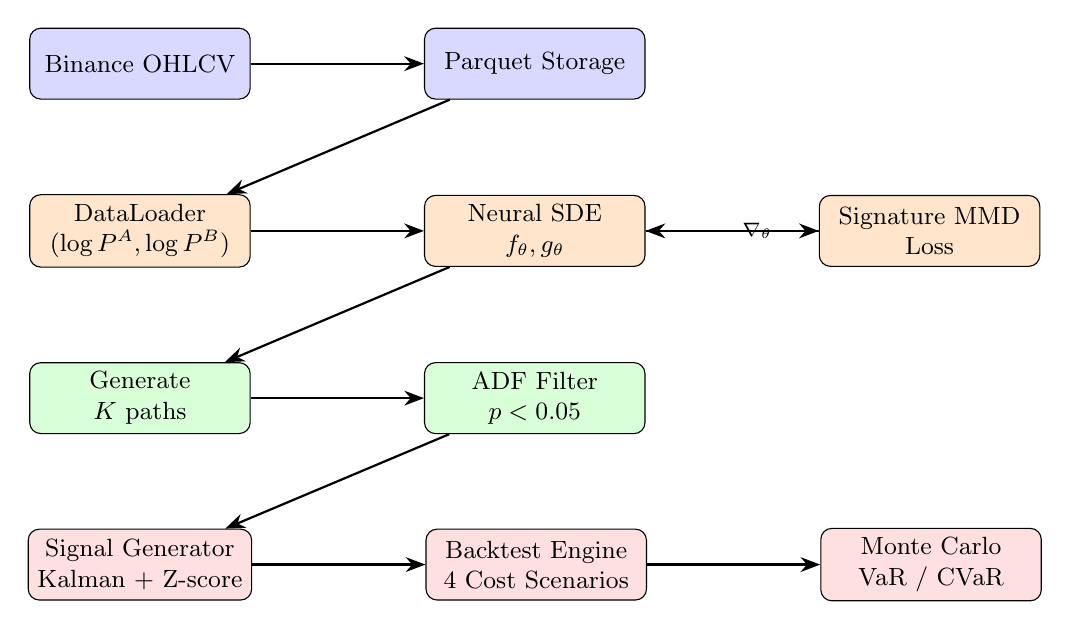
\begin{tikzpicture}[
    node distance=1.2cm and 2.2cm,
    block/.style={rectangle, draw, rounded corners, minimum width=2.8cm, minimum height=0.9cm, align=center, font=\small},
    arrow/.style={-{Stealth[length=2.5mm]}, thick},
]
    % Data layer
    \node[block, fill=blue!15] (binance) {Binance OHLCV};
    \node[block, fill=blue!15, right=of binance] (parquet) {Parquet Storage};
    
    % Neural SDE
    \node[block, fill=orange!20, below=of binance] (dataloader) {DataLoader\\$(\log P^A, \log P^B)$};
    \node[block, fill=orange!20, right=of dataloader] (sde) {Neural SDE\\$f_\theta, g_\theta$};
    \node[block, fill=orange!20, right=of sde] (sigmmd) {Signature MMD\\Loss};
    
    % Generation
    \node[block, fill=green!15, below=of dataloader] (generate) {Generate\\$K$ paths};
    \node[block, fill=green!15, right=of generate] (adf) {ADF Filter\\$p < 0.05$};
    
    % Backtest
    \node[block, fill=red!12, below=of generate] (signal) {Signal Generator\\Kalman + Z-score};
    \node[block, fill=red!12, right=of signal] (backtest) {Backtest Engine\\4 Cost Scenarios};
    \node[block, fill=red!12, right=of backtest] (montecarlo) {Monte Carlo\\VaR / CVaR};
    
    % Arrows
    \draw[arrow] (binance) -- (parquet);
    \draw[arrow] (parquet) -- (dataloader);
    \draw[arrow] (dataloader) -- (sde);
    \draw[arrow] (sde) -- (sigmmd);
    \draw[arrow, dashed] (sigmmd) -- node[right, font=\scriptsize] {$\nabla_\theta$} (sde);
    \draw[arrow] (sde) -- (generate);
    \draw[arrow] (generate) -- (adf);
    \draw[arrow] (adf) -- (signal);
    \draw[arrow] (signal) -- (backtest);
    \draw[arrow] (backtest) -- (montecarlo);
\end{tikzpicture}
\caption{End-to-end pipeline: from raw data ingestion to Monte Carlo risk evaluation.}
\label{fig:pipeline}
\end{figure}

% ============================================================
\section{Implementation Details}
\label{sec:impl}
% ============================================================

\begin{table}[h]
\centering
\caption{Hyperparameters used in experiments.}
\label{tab:hyperparams}
\begin{tabular}{@{}lll@{}}
\toprule
\textbf{Component} & \textbf{Parameter} & \textbf{Value} \\
\midrule
\multirow{3}{*}{Neural SDE} 
    & State dimension $d$ & 2 \\
    & Hidden dimension $H$ & 64 \\
    & Target volatility $\sigma_{\text{target}}$ & 1.0 \\
\midrule
\multirow{6}{*}{Training}
    & Sequence length $L$ & 256 \\
    & Stride $\Delta$ & 8 \\
    & Batch size $B$ & 128 \\
    & Signature depth $N_s$ & 3 \\
    & Learning rate & $10^{-3}$ (AdamW) \\
    & Weight decay & $10^{-2}$ \\
    & Early stopping patience & 70 epochs \\
    & Integration method & Milstein \\
\midrule
\multirow{3}{*}{Data}
    & Asset pair & ADA/USDT $\times$ AVAX/USDT \\
    & Timeframe & 1 hour \\
    & Train/Val split & 80\% / 20\% (chronological) \\
\bottomrule
\end{tabular}
\end{table}

The model is trained on AWS EC2 Spot instances (g4dn.xlarge) with CUDA acceleration. Training telemetry is logged via Weights~\&~Biases. The codebase uses \texttt{torchsde} for SDE integration and \texttt{signatory} for GPU-accelerated signature computation.

% ============================================================
\section{Discussion}
\label{sec:discussion}
% ============================================================

\paragraph{Why Neural SDE over autoregressive models?}
Autoregressive generative models (e.g., GPT-style, or our previous Conditional Flow Matching approach) generate paths as sequences of discrete steps, requiring \emph{stitching} for long-horizon generation. The SDE formulation integrates continuously, producing paths of arbitrary length in a single forward solve without accumulating stitching artifacts.

\paragraph{Why distributional matching via signatures?}
Pointwise losses (MSE on returns, log-likelihood) match individual trajectories but do not guarantee that the \emph{distribution} of generated paths matches reality. The Kernel Signature MMD operates on the space of path measures, ensuring that all continuous functionals of the path --- including volatility clustering, autocorrelation structure, and tail behavior --- are replicated.

\paragraph{Role of spread deviation conditioning.}
Without $\Delta s_t$, the drift and diffusion networks would need to implicitly learn the cointegration relationship from the two log-prices alone. By explicitly providing the spread deviation as an auxiliary input, we inject domain knowledge about mean-reversion into the architecture, significantly reducing the sample complexity of training.

% ============================================================
\section{Conclusion}
\label{sec:conclusion}
% ============================================================

We have presented a Neural SDE framework for generating synthetic cointegrated market paths to stress-test pairs trading strategies. The key innovations are:
\begin{enumerate}[nosep]
    \item \emph{Spread deviation conditioning}: encoding mean-reversion directly in the SDE architecture.
    \item \emph{Kernel Signature MMD training}: distributional matching in the universal feature space of path signatures.
    \item \emph{ADF quality filtering}: post-generation stationarity enforcement for robust Monte Carlo evaluation.
\end{enumerate}

This framework transforms the model evaluation paradigm from ``how did the strategy perform on one historical path?'' to ``what is the distribution of strategy performance across thousands of plausible market scenarios?'', enabling statistically rigorous risk assessment.

% ============================================================
% References
% ============================================================
\bibliographystyle{plainnat}
\begin{thebibliography}{10}

\bibitem[Kidger et~al.(2021)]{kidger2021neural}
P.~Kidger, J.~Foster, X.~Li, and T.~Lyons.
\newblock Neural {SDEs} as infinite-dimensional {GANs}.
\newblock In \emph{Proceedings of the 38th International Conference on Machine Learning (ICML)}, 2021.

\bibitem[Lyons(1998)]{lyons1998differential}
T.~Lyons.
\newblock Differential equations driven by rough paths.
\newblock \emph{Revista Matem\'atica Iberoamericana}, 14(2):215--310, 1998.

\bibitem[Kir\'aly and Oberhauser(2019)]{kiraly2019kernels}
F.~Kir\'aly and H.~Oberhauser.
\newblock Kernels for sequentially ordered data.
\newblock \emph{Journal of Machine Learning Research}, 20(31):1--45, 2019.

\bibitem[Kloeden and Platen(1992)]{kloeden1992numerical}
P.~E. Kloeden and E.~Platen.
\newblock \emph{Numerical Solution of Stochastic Differential Equations}.
\newblock Springer-Verlag, 1992.

\bibitem[Vidyamurthy(2004)]{vidyamurthy2004pairs}
G.~Vidyamurthy.
\newblock \emph{Pairs Trading: Quantitative Methods and Analysis}.
\newblock Wiley, 2004.

\bibitem[Chevyrev and Oberhauser(2022)]{chevyrev2022signature}
I.~Chevyrev and H.~Oberhauser.
\newblock Signature moments to characterize laws of stochastic processes.
\newblock \emph{Journal of Machine Learning Research}, 23(176):1--42, 2022.

\bibitem[Gretton et~al.(2012)]{gretton2012kernel}
A.~Gretton, K.~M. Borgwardt, M.~J. Rasch, B.~Sch\"olkopf, and A.~Smola.
\newblock A kernel two-sample test.
\newblock \emph{Journal of Machine Learning Research}, 13:723--773, 2012.

\end{thebibliography}

\end{document}
